\iffalse
This file is protected by Copyright. Please refer to the COPYRIGHT file
distributed with this source distribution.

This file is part of OpenCPI <http://www.opencpi.org>

OpenCPI is free software: you can redistribute it and/or modify it under the
terms of the GNU Lesser General Public License as published by the Free Software
Foundation, either version 3 of the License, or (at your option) any later
version.

OpenCPI is distributed in the hope that it will be useful, but WITHOUT ANY
WARRANTY; without even the implied warranty of MERCHANTABILITY or FITNESS FOR A
PARTICULAR PURPOSE. See the GNU Lesser General Public License for more details.

You should have received a copy of the GNU Lesser General Public License along
with this program. If not, see <http://www.gnu.org/licenses/>.
\fi

%----------------------------------------------------------------------------------------
% Update the docTitle and docVersion per document
%----------------------------------------------------------------------------------------
\def\docTitle{OpenCPI\\ FSK App Guide\\ (E310 Supplement)}
\def\docVersion{1.5}
%----------------------------------------------------------------------------------------
% AV-5479: Assume this is in projects/bsps/XXX of source checkout
\def\snippetpath{../../../../../../doc/av/tex/snippets}
\input{\snippetpath/includes}
\documentclass{article}
\iffalse
This file is protected by Copyright. Please refer to the COPYRIGHT file
distributed with this source distribution.

This file is part of OpenCPI <http://www.opencpi.org>

OpenCPI is free software: you can redistribute it and/or modify it under the
terms of the GNU Lesser General Public License as published by the Free Software
Foundation, either version 3 of the License, or (at your option) any later
version.

OpenCPI is distributed in the hope that it will be useful, but WITHOUT ANY
WARRANTY; without even the implied warranty of MERCHANTABILITY or FITNESS FOR A
PARTICULAR PURPOSE. See the GNU Lesser General Public License for more details.

You should have received a copy of the GNU Lesser General Public License along
with this program. If not, see <http://www.gnu.org/licenses/>.
\fi
% Any changes to this document should be made in opencpi.git
\author{} % Force author to be blank
%----------------------------------------------------------------------------------------
% Paper size, orientation and margins
%----------------------------------------------------------------------------------------
\usepackage{geometry}
\geometry{
        letterpaper, % paper type
        portrait,    % text direction
        left=.75in,  % left margin
        top=.75in,   % top margin
        right=.75in, % right margin
        bottom=.75in % bottom margin
 }
%----------------------------------------------------------------------------------------
% Header/Footer
%----------------------------------------------------------------------------------------
\usepackage{fancyhdr} \pagestyle{fancy} % required for fancy headers
\renewcommand{\headrulewidth}{0.5pt}
\renewcommand{\footrulewidth}{0.5pt}
\rhead{\small{ANGRYVIPER Team}}
% \rfoot{\thepage}
%----------------------------------------------------------------------------------------
% Appendix packages
%----------------------------------------------------------------------------------------
\usepackage[toc,page]{appendix}
%----------------------------------------------------------------------------------------
% Defined Commands & Renamed Commands
%----------------------------------------------------------------------------------------
\renewcommand{\contentsname}{Table of Contents}
\renewcommand{\listfigurename}{List of Figures}
\renewcommand{\listtablename}{List of Tables}
\newcommand{\todo}[1]{\textcolor{red}{TODO: #1}\PackageWarning{TODO:}{#1}} % To do notes
\newcommand{\code}[1]{\texttt{#1}} % For inline code snippet or command line
%----------------------------------------------------------------------------------------
% Various packages
%----------------------------------------------------------------------------------------
\usepackage[usenames,dvipsnames]{xcolor} % for color names see https://en.wikibooks.org/wiki/LaTeX/Colors
\usepackage{hyperref}  % for linking urls and lists
\usepackage{graphicx}  % for including pictures by file
\usepackage{listings}  % for coding language styles
\usepackage{rotating}  % for sideways table
\usepackage{pifont}    % for sideways table
\usepackage{pdflscape} % for landscape view
\usepackage{subfig}
\hyphenation{ANGRY-VIPER} % Tell it where to hyphenate
\hyphenation{Cent-OS} % Tell it where to hyphenate
\hyphenation{install-ation} % Tell it where to hyphenate
\uchyph=0 % Never hyphenate acronyms like RCC (I think this overrides ANGRYVIPER above)
\renewcommand\_{\textunderscore\allowbreak} % Allow words to break/newline on underscores
%----------------------------------------------------------------------------------------
% Table packages
%----------------------------------------------------------------------------------------
\usepackage{longtable} % for long possibly multi-page tables
\usepackage{tabularx} % c=center,l=left,r=right,X=fill
% These define tabularx columns "C" and "R" to match "X" but center/right aligned
\newcolumntype{C}{>{\centering\arraybackslash}X}
\newcolumntype{R}{>{\raggedleft\arraybackslash}X}
\usepackage{float}
\floatstyle{plaintop}
\usepackage[tableposition=top]{caption}
\newcolumntype{P}[1]{>{\centering\arraybackslash}p{#1}}
\newcolumntype{M}[1]{>{\centering\arraybackslash}m{#1}}
%----------------------------------------------------------------------------------------
% Block Diagram / FSM Drawings
%----------------------------------------------------------------------------------------
\usepackage{tikz}
\usetikzlibrary{shapes,arrows,fit,positioning}
\usetikzlibrary{automata} % used for the fsm
%----------------------------------------------------------------------------------------
% Colors Used
%----------------------------------------------------------------------------------------
\usepackage{colortbl}
\definecolor{blue}{rgb}{.7,.8,.9}
\definecolor{ceruleanblue}{rgb}{0.16, 0.32, 0.75}
\definecolor{drkgreen}{rgb}{0,0.6,0}
\definecolor{deepmagenta}{rgb}{0.8, 0.0, 0.8}
\definecolor{cyan}{rgb}{0.0,0.6,0.6}
\definecolor{maroon}{rgb}{0.5,0,0}
%----------------------------------------------------------------------------------------
% VHDL Coding Language Style
% modified from: http://latex-community.org/forum/viewtopic.php?f=44&t=22076
%----------------------------------------------------------------------------------------
\lstdefinelanguage{VHDL}
{
        basicstyle=\ttfamily\footnotesize,
        columns=fullflexible,keepspaces,      % https://tex.stackexchange.com/a/46695/87531
        keywordstyle=\color{ceruleanblue},
        commentstyle=\color{drkgreen},
        morekeywords={
    library,use,all,entity,is,port,in,out,end,architecture,of,
    begin,and, signal, when, if, else, process, end,
        },
        morecomment=[l]--
}
%----------------------------------------------------------------------------------------
% XML Coding Language Style
% modified from: http://tex.stackexchange.com/questions/10255/xml-syntax-highlighting
%----------------------------------------------------------------------------------------
\lstdefinelanguage{XML}
{
        basicstyle=\ttfamily\footnotesize,
        columns=fullflexible,keepspaces,
        morestring=[s]{"}{"},
        morecomment=[s]{!--}{--},
        commentstyle=\color{drkgreen},
        moredelim=[s][\color{black}]{>}{<},
        moredelim=[s][\color{cyan}]{\ }{=},
        stringstyle=\color{maroon},
        identifierstyle=\color{ceruleanblue}
}
%----------------------------------------------------------------------------------------
% DIFF Coding Language Style
% modified from http://tex.stackexchange.com/questions/50176/highlighting-a-diff-file
%----------------------------------------------------------------------------------------
\lstdefinelanguage{diff}
{
        basicstyle=\ttfamily\footnotesize,
        columns=fullflexible,keepspaces,
        breaklines=true,                                % wrap text
        morecomment=[f][\color{ceruleanblue}]{@@},      % group identifier
        morecomment=[f][\color{red}]-,                  % deleted lines
        morecomment=[f][\color{drkgreen}]+,             % added lines
        morecomment=[f][\color{deepmagenta}]{---},      % Diff header lines (must appear after +,-)
        morecomment=[f][\color{deepmagenta}]{+++},
}
%----------------------------------------------------------------------------------------
% Python Coding Language Style
% modified from
%----------------------------------------------------------------------------------------
\lstdefinelanguage{python}
{
        basicstyle=\ttfamily\footnotesize,
        columns=fullflexible,keepspaces,
        keywordstyle=\color{ceruleanblue},
        commentstyle=\color{drkgreen},
        stringstyle=\color{orange},
        morekeywords={
    print, if, sys, len, from, import, as, open,close, def, main, for, else, write, read, range,
        },
        comment=[l]{\#}
}
%----------------------------------------------------------------------------------------
% Fontsize Notes in order from smallest to largest
%----------------------------------------------------------------------------------------
%    \tiny
%    \scriptsize
%    \footnotesize
%    \small
%    \normalsize
%    \large
%    \Large
%    \LARGE
%    \huge
%    \Huge

\date{Version \docVersion} % Force date to be blank and override date with version
\title{\docTitle}
\lhead{FSK App Guide}
%----------------------------------------------------------------------------------------
%\usepackage[T1]{fontenc} % http://tex.stackexchange.com/a/181119
\usepackage{graphicx}
\graphicspath{ {figures/} }
\usepackage{textcomp}

\begin{document}
\maketitle
%\thispagestyle{fancy}
\newpage
	\begin{center}
	\textit{\textbf{Revision History}}
		\begin{table}[H]
		\label{table:revisions} % Add "[H]" to force placement of table
			\begin{tabularx}{\textwidth}{|c|X|l|}
			\hline
			\rowcolor{blue}
			\textbf{Revision} & \textbf{Description of Change} & \textbf{Date} \\
			\hline
			v1.3.1-E3XX & Updated for E310 support & 3/2018 \\
			\hline
			v1.4 & Updated with simplications and references to assets' document & 9/2018 \\
			\hline
			v1.5 & Version bump only & 4/2019 \\
			\hline
			\end{tabularx}
		\end{table}
	\end{center}

\newpage
\tableofcontents
\pagebreak
\def\assetsdoc{\noindent For more information on this application, see \code{ocpi.assets}'s more in-depth version of the \textit{FSK\_app} document.}
\section{Document Scope}
This document describes the OpenCPI FSK demo application. It includes a description of the application, instructions to setup the hardware, build of bitstreams, and execution of the application itself on various platforms.

\section{Description}
\assetsdoc

\section{Hardware Portability}
This application is specific to the \verb+e3xx+ platform.

\section{Building the Application}
\subsection{Dependencies}
\noindent The tables below breakdown the workers used within the various platforms and modes of the FSK App. Appendix A shows the exact worker configurations used in the HDL assemblies. See the individual component data sheets for more information and build instructions. Similarly, the HDL platform worker and configurations for the intended radio must be compiled prior to building the various FSK bitstreams.
\subsection{FSK Mode Configurations}
\subsubsection{Common to all Hardware}
	\begin{tabular}{|c|c|c|c|c|c|}
	\hline
	\rowcolor{blue}
	Application XML & filerw & rx & tx & txrx & bbloopback \\
	\hline
	app\_fsk\_filerw (dependency only, no build required) & x & • & • & • & • \\
	\rowcolor{blue}
	HDL Assemblies & filerw & rx & tx & txrx & bbloopback \\
	\hline
	fsk\_filerw & x & • & • & • & • \\
	\hline
	dc\_offset\_iq\_imbalance\_mixer\_cic\_dec\_rp\_cordic\_fir\_real & • & x & • & • & • \\
	\hline
	mfsk2\_zp16\_fir\_real\_phase\_to\_amp\_cordic\_cic\_int & • & • & x & • & • \\
	\hline
	fsk\_modem & • & • & • & x & x \\
	\hline
	\rowcolor{blue}
	RX Path Workers & filerw & rx & tx & txrx & bbloopback \\
	\hline
	dc\_offset\_filter.hdl & • & x & • & x & x \\
	\hline
	iq\_imbalance\_fixer.hdl & • & x & • & x & x \\
	\hline
	complex\_mixer.hdl & x & x & • & x & x \\
	\hline
	cic\_dec.hdl & x & x & • & x & x \\
	\hline
	rp\_cordic.hdl & x & x & • & x & x \\
	\hline
	fir\_real\_sse.hdl & x & x & • & x & x \\
	\hline
	baudTracking.rcc & x & x & • & x & x \\
	\hline
	real\_digitizer.rcc & x & x & • & x & x \\
	\hline
	file\_write.rcc & x & x & • & x & x \\
	\hline
	\rowcolor{blue}
	TX Path Workers & filerw & rx & tx & txrx & bbloopback \\
	\hline
	file\_read.rcc & x & • & x & x & x \\
	\hline
	mfsk\_mapper.hdl & x & • & x & x & x \\
	\hline
	zero\_pad.hdl & x & • & x & x & x \\
	\hline
	fir\_real\_sse.hdl & x & • & x & x & x \\
	\hline
	phase\_to\_amp\_cordic.hdl & x & • & x & x & x \\
	\hline
	cic\_int.hdl & x & • & x & x & x \\
	\hline
	\end{tabular}

\subsubsection{Additional Dependencies for Ettus E310}
	\begin{tabular}{|c|c|c|c|c|c|}
	\hline
	\rowcolor{blue}
	Application XML & filerw & rx & tx & txrx & bbloopback \\
	\hline
	app\_fsk\_rx\_e3xx (dependency only, no build required) & • & x & • & • & • \\
	\hline
	app\_fsk\_tx\_e3xx (dependency only, no build required) & • & • & x & • & • \\
	\hline
	app\_fsk\_txrx\_e3xx (dependency only, no build required) & • & •  & • & x & • \\
	\hline
	\rowcolor{blue}
	RX or TX Path Workers & filerw & rx & tx & txrx & bbloopback \\
	\hline
	ad9361\_data\_sub.hdl & • & x & x & x & • \\
	\rowcolor{blue}
	RX Path Workers & filerw & rx & tx & txrx & bbloopback \\
	\hline
	ad9361\_adc.hdl & • & x & • & x & • \\
	\hline
	ad9361\_adc\_sub.hdl & • & x & • & x & • \\
	\hline
	\rowcolor{blue}
	TX Path Workers & filerw & rx & tx & txrx & bbloopback \\
	\hline
	ad9361\_dac.hdl & • & • & x & x & • \\
	\hline
	ad9361\_dac\_sub.hdl & • & • & x & x & • \\
	\rowcolor{blue}
	Endpoint Proxies & filerw & rx & tx & txrx & bbloopback \\
	\hline
	e3xx\_rx.rcc & • & x & • & x & • \\
	\hline
	e3xx\_tx.rcc & • & • & x & x & • \\
	\hline
	\rowcolor{blue}
	SPI Command and Control & filerw & rx & tx & txrx & bbloopback \\
	\hline
	ad9361\_config.hdl & • & x & x & x & • \\
	\hline
	ad9361\_config\_proxy.rcc & • & x & x & x & •  \\
	\hline
	ad9361\_spi.hdl & • & x & x & x &   \\
	\hline
	e3xx\_mimo\_xcvr\_ad5662.hdl & • & x & x & x &   \\
	\hline
	\rowcolor{blue}
	I2C Command and Control & filerw & rx & tx & txrx & bbloopback \\
	\hline
	e3xx\_i2c.hdl & • & x & x & x &   \\
	\hline
	\rowcolor{blue}
	Analog Filter Control & filerw & rx & tx & txrx & bbloopback \\
	\hline
	e3xx\_mimo\_xcvr\_filter.hdl & • & x & x & x &   \\
	\hline
	e3xx\_mimo\_xcvr\_filter\_proxy.rcc & • & x & x & x &   \\
	\hline
	\end{tabular}

	\newpage
\subsection{HDL Assembly and HDL Container}
\assetsdoc

\begin{landscape}
\subsection{Performance and Resource Utilization}
\subsubsection{filerw}
\assetsdoc
\subsubsection{tx}
\input{../../../hdl/assemblies/mfsk2_zp16_fir_real_phase_to_amp_cordic_cic_int/utilization.inc}
\subsubsection{rx}
\input{../../../hdl/assemblies/dc_offset_iq_imbalance_mixer_cic_dec_rp_cordic_fir_real/utilization.inc}
\subsubsection{txrx/bbloopback}
\input{../../../hdl/assemblies/fsk_modem/utilization.inc}
\end{landscape}
\subsection{Executable}
\noindent To build for the Ettus E310 (which runs the xilinx13\_4 PetaLinux operating system), run the following command from the FSK directory:\par\medskip
\texttt{ ocpidev build --rcc-platform xilinx13\_4 }\par\medskip
\assetsdoc

\section{Testing the Application}
\assetsdoc
\subsection{make show}
In order to test the application using the various modes mentioned above, \texttt{make show} can be run from the \texttt{applications/FSK} directory. This provides instructions (for Zynq-Based Platforms) for setting \texttt{OCPI\_LIBRARY\_PATH} on the hardware platform and then running the application. Finally, it explains how to verify the output data on the development computer. The following sections provide further insight into these instructions.
\subsection{Artifacts}
\assetsdoc \\
\noindent Appendix B includes a list of the artifacts required for each platform and mode.
\subsection{Arguments to executable}
\assetsdoc \\
\noindent Example arguments for the \textbf{Ettus E310 BSP} using the SMA ports RX=RX2A TX=TRXA:\\
\begin{tabular}{|l|l|}
\hline
\rowcolor{blue}
Parameter 	&        Value  	\\
\hline
RF frontend 	&        (not set / default)  	\\
\hline
Runtime (s) 	&        20 	        \\
\hline
RX SMA channel 	&        RX2A              	\\
\hline
TX SMA channel 	&        TRXA           	\\
\hline
rx\_sample\_rate 	&4 	                \\
\hline
rx\_rf\_center\_freq 	&2400  	\\
\hline
rx\_rf\_bw 	&        -1 (default)   \\
\hline
rx\_rf\_gain 	&        12       	\\
\hline
rx\_bb\_bw 	&        4 	        \\
\hline
rx\_bb\_gain 	&        -1 (default) 	\\
\hline
rx\_if\_center\_freq 	&0              	\\
\hline
tx\_sample\_rate 	&4              	\\
\hline
tx\_rf\_center\_freq 	&2400 	        \\
\hline
tx\_rf\_bw 	&        -1 (default)   \\
\hline
tx\_rf\_gain 	&        -28 	        \\
\hline
tx\_bb\_bw 	&        4        	\\
\hline
tx\_bb\_gain    &       -1 (default) \\
\hline
\end{tabular}\par\medskip

\noindent Note that if the application complains about the output file or directory, run `\code{mkdir odata}' in the FSK directory and rerun the executable.
\pagebreak
\subsection{Library Path Requirements}
\noindent Prior to running the application, the environment variable OCPI\_LIBRARY\_PATH must be configure, such that, all of the FSK application's run-time artifacts can be located. OpenCPI conveniently provides access to a project's run-time artifacts at the top-level of each project in a directory called artifacts. Reference the OpenCPI Application Development Guide for more about OCPI\_LIBRARY\_PATH. \par\medskip

\noindent Examples of library paths that could be used can be seen below:\\

\noindent The following are recommendations for configuring the OCPI\_LIBRARY\_PATH based on the platform, the use of a daughter card and specific slot that card is installed. For all recommendations:
\begin{itemize}
  \item All paths are relative to the applications/rx\_app/ directory.\\
\end{itemize}

\noindent\textbf{Recommended Library Path}\\
\noindent
Follow the instructions contained in the FSK application's Makefile. They can be viewed by opening the Makefile in an editor, or by executing ``make show'' from within the assets/applications/FSK/.\\

\pagebreak

\subsection{Expected results}
\noindent In the case of the \textit{filerw}, \textit{rx}, \textit{txrx}, and \textit{bbloopback} modes, assuming transmission of the idata/Os.jpeg input file, the expected result is a transmitted copy of the JPEG file. A Linux program such as Eye of GNOME (eog) may be used to display the JPEG file. The file is shown in Figure \ref{fig:os_pic}.\par\medskip
\noindent In the case of the \textit{tx} mode, verification is obtained by viewing the RF spectrum on a spectrum analyzer. An example of the transmitted spectrum may be seen in Figure \ref{fig:tx_spec_an}.\par\medskip
	\begin{figure}[ht]
	 	\centering
	 	\begin{minipage}{.325\textwidth}
			\centering\includegraphics[width=1.0\linewidth]{Os}
			\caption{FSK input file}
			\label{fig:os_pic}
		\end{minipage}
	 	\begin{minipage}{.45\textwidth}
			\centering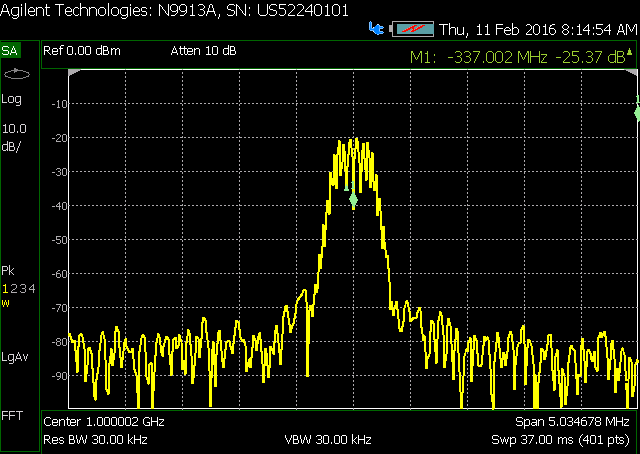
\includegraphics[width=1.0\linewidth]{tx_spec_an}
			\caption{Output of FSK App RF transmit}
			\label{fig:tx_spec_an}
		\end{minipage}
	\end{figure}
\pagebreak
\subsection{Known Issues}
\noindent
\begin{itemize}
  \item The \textit{rx} and \textit{tx} modes suffer from limited carrier recovery ability. The requested center frequency may need to be adjusted to a value other than the exact expected nominal value.
  \item Sometimes the radio can get into an unwanted state. If unusual results are seen, run \code{ocpihdl unload} and rerun the application.
\end{itemize}

\pagebreak
\section{Appendix A: Worker Parameters}
Configuration information for each component in the application can be found in the application XML for that configuration. \textit{E.g.} for the Ettus E310 in txrx mode, \code{app\_fsk\_txrx\_e3xx}. Further information can be determined by browsing the chosen platform configurations and container XMLs for the given configuration and platform.
\section{Appendix B: Artifacts}
Each worker that is required for a given configuration of this application has an artifact that must be found at runtime (located via one of the \code{OCPI\_LIBRARAY\_PATH} choices listed above). Reference the lists of workers for each configuration and platform to determine the artifacts required. Each required RCC worker corresponds to a required \\
\code{target-<shortened-rcc-platform>/<worker>\_s.so} artifact. All required HDL workers (together) correspond to a single required \code{<assembly>\_<platform>\_<platform-config>\_<container>.bitz} artifact.\\
\subsection{Ettus E310}
	\noindent\textbf{filerw}
	\begin{itemize}
	\begin{minipage}[t]{.5\textwidth}
	\item fsk\_filerw\_e3xx\_base.bitz

	\item target-xilinx13\_4/file\_read\_s.so
	\item target-xilinx13\_4/Baudtracking\_simple\_s.so
	\end{minipage}
	\begin{minipage}[t]{.5\textwidth}
	\item target-xilinx13\_4/real\_digitizer\_s.so
	\item target-xilinx13\_4/file\_write\_s.so
	\end{minipage}
	\end{itemize}

	\noindent\textbf{rx}
	\begin{itemize}
  \item dc\_offset\_iq\_imbalance\_mixer\_cic\_dec\_rp\_cordic\_fir\_real\_e3xx\_cfg\_1rx\_0tx\_mode\_2\_cmos\_cnt\_1rx\_0tx\_mode\_2\_ \\
	bypassasm\_e3xx\_mimo\_xcvr\_CMOS\_e3xx.bitz \\

	\begin{minipage}[t]{.5\textwidth}
	\item target-xilinx13\_4/Baudtracking\_simple\_s.so
	\item target-xilinx13\_4/real\_digitizer\_s.so
	\item target-xilinx13\_4/file\_write\_s.so
	\end{minipage}
	\begin{minipage}[t]{.5\textwidth}
	\item target-xilinx13\_4/ad9361\_config\_proxy\_s.so
	\item target-xilinx13\_4/e3xx\_mimo\_xcvr\_filter\_proxy\_s.so
	\item target-xilinx13\_4/e3xx\_rx\_s.so
	\end{minipage}
	\end{itemize}

	\noindent\textbf{tx}
	\begin{itemize}
  \item mfsk2\_zp16\_fir\_real\_phase\_to\_amp\_cordic\_cic\_int\_e3xx\_cfg\_0rx\_1tx\_mode\_2\_cmos\_cnt\_0rx\_1tx\_mode\_2\_thruasm\_ \\
	e3xx\_mimo\_xcvr\_CMOS\_e3xx.bitz \\

	\begin{minipage}[t]{.5\textwidth}
	\item target-xilinx13\_4/file\_read\_s.so
	\item target-xilinx13\_4/ad9361\_config\_proxy\_s.so
	\end{minipage}
	\begin{minipage}[t]{.5\textwidth}
	\item target-xilinx13\_4/e3xx\_mimo\_xcvr\_filter\_proxy\_s.so
	\item target-xilinx13\_4/e3xx\_tx\_s.so
	\end{minipage}
	\end{itemize}

	\noindent\textbf{txrx/bbloopback}
	\begin{itemize}
  \item fsk\_modem\_e3xx\_cfg\_1rx\_1tx\_mode\_2\_cmos\_cnt\_1rx\_1tx\_mode\_2\_thruasm\_e3xx\_mimo\_xcvr\_CMOS\_e3xx.bitz \\

	\begin{minipage}[t]{.5\textwidth}
	\item target-xilinx13\_4/file\_read\_s.so
	\item target-xilinx13\_4/Baudtracking\_simple\_s.so
	\item target-xilinx13\_4/real\_digitizer\_s.so
	\end{minipage}
	\begin{minipage}[t]{.5\textwidth}
	\item target-xilinx13\_4/file\_write\_s.so
	\item target-xilinx13\_4/ad9361\_config\_proxy\_s.so
	\item target-xilinx13\_4/e3xx\_mimo\_xcvr\_filter\_proxy\_s.so
	\item target-xilinx13\_4/e3xx\_rx\_s.so
	\item target-xilinx13\_4/e3xx\_tx\_s.so
	\end{minipage}
	\end{itemize}




\end{document}
